\section{Methods}
\subsection{A suitable smoothness metric for binding site prediction}
There has been some work on smoothness of labels or features over graphs using some form of measure
of local variations around each vertex as a smoothness metric
\citep{zhou2004regularization,hou2019measuring,wang2019knowledge}. However, the smoothness metrics
used by most of these works are not suitable for imbalanced classes. In our case, since binding site
regions are generally only a small portion of the whole protein surface, the classes are extremely
imbalanced. This means, metrics not addressing class imbalance all give extremely high values of
smoothness even for meshes which we would consider as quite "unsmooth" due to lots of
patchy/scattered predictions. 
\par
Given a graph $G=(V, E)$ and label assignments $l$ such that $l_v \in \{0, 1, ..., k-1\} \forall v\in V$,
an example of a smoothness metric not considering class imbalance is as follows:
\begin{align*}
        M_1 &= \frac{1}{|E|} \sum_{(u,v) \in E}\bI[l_u = l_v]\numberthis \label{simple_smoothness}
\end{align*}
The metric $M_1$ presented above has a value of 1 if all the labels belong to one class and has a 
value around 0.5 when the labels are totally randomly assigned. This already limits the
range of this metric. Not only that in practice, we almost never see  our predicted labels over protein
meshes go below the value of 0.9. Which makes the metric really skewed and any judgements of
improvements in similarity is difficult to make. There are other weighted versions of this metric
possible, for example, an inverse edge weighted version we attempted looks as follows:
\begin{align*}
        M_2 &= 1 - \frac{1}{\sum_{(u,v) \in E}\frac{1}{d(u,v)}} \sum_{(u,v) \in
        E}\frac{1}{d(u,v)}\bI[l_u \neq l_v]\numberthis \label{inverse_edge_weghted_smoothness}\\
        where, d(u,v) &= \text{ distance between vertices $u,v$ or edge length of $(u,v)$}
\end{align*}
However, this does not help much, because the variance of the edge length distribution
is really low for our protein meshes. So, it behaves similarly as $M_1$.
\par
So finally, we designed a metric which takes care of the issue of label imbalanced (and the
resulting skewed smoothness values). Assuming there are $k$ possible classes, we computing a measure
of smoothness for labels corresponding to each of these classes separately and then do a weighted
combination of them. So, let, $V_i \subset V$ be the set of vertices which has the label $i \in
\{0,1,..,k-1\}$, and $V_i^{in} \subset V_i$ to be the set of vertices within $V_i$ all of whose
neighbours have class label $i$. This makes $V_i^{out} = V - V_i^{in}$ the vertices which have at
least one neighbour having a class label other than $i$. So, in essence, $V_i^{in}$ is analogous to
area and $V_i^{out}$ is analogous to the perimeter of regions with class label $i$. Hence, a measure for
smoothness for class $i$ is simply:
\begin{align*}
        S_i = \frac{|V_i^{in}|}{|V_i|} = 1 - \frac{|V_i^{out}|}{|V_i|} \numberthis \\
\end{align*}
Now, we can take weighted combination of these class specific metrics to constitute a balanced
smoothness smoothness metric:
\begin{align*}
        S = \frac{\sum_{i = 0}^{k-1}\frac{1}{|V_i|}S_i}{\sum_{i = 0}^{k-1}\frac{1}{|V_i|}} =
        \frac{\sum_{i = 0}^{k-1}\frac{|V_i^{in}|}{|V_i|^2}}{\sum_{i = 0}^{k-1}\frac{1}{|V_i|}} \numberthis \label{final_smoothness_metric}
\end{align*}
This metric is nice in the sense it gives a broader range of values and
hence is more useful in our case. In \hyperref[fig:smooth]{Fig. 1.2} we show how the metrics $M1$,  $M2$, $S$ behave by applying it on a set of 15 different proteins with predicted labels by PNAbind. This demonstrates the advantage of $S$ clearly over the other two metrics.
\subsection{Continuous Conditional Random Fields layer}
Given a graph $G = (V,E)$, features over graph vertices $x$ such that $x_v \in \bR^d \forall v \in V
$ and labels over the vertices $y$ such that $y_v \in \{0,1,..,k\} \forall v
\in V$, A CRF aims to maximize the following probability to reassign the labels $y$.
\begin{align*}
        P(y_i | x, y_{j\neq i} ) &= 
        \frac{1}{Z(x_i)} exp [- (\psi_1(x_i,y_i) + \sum_{j \in
        \cN(i)}\psi_2(y_i,y_j,x_i,x_j)) ] \numberthis \label{crf_general}
\end{align*}
The terms $\psi_1$ and $\psi_2$ in the above equation are known as unary and binary potentials
respectively. $\psi_1$ models how much the label $y_i$ conforms to the features $x_i$ and $\psi_2$
models how much the label $y_i$ conforms to the labels and features of the neighbours of vertex $i$.
The exact form of these terms can be application dependent and designed accordingly. 
However, optimizing eq. \ref{crf_general} in a general scenario is non-trivial and approximations
either do not perform well or are heavily resource consuming. Moreover, this kind of optimization over
discrete domain is not suitable for neural network application. 
\par
In our case, PNAbind is a deep learning model. So , we would like to implement this conditional random field 
model as a network layer which can just be plugged into the network and will be optimized by backpropagation 
along with the whole network, without us requiring any extra optimization. So, following the
approach described in \citet{gao2019conditional, ristovski2013continuous} we instead use a
Continuous CRF model. 
\begin{figure}[H]
\centering
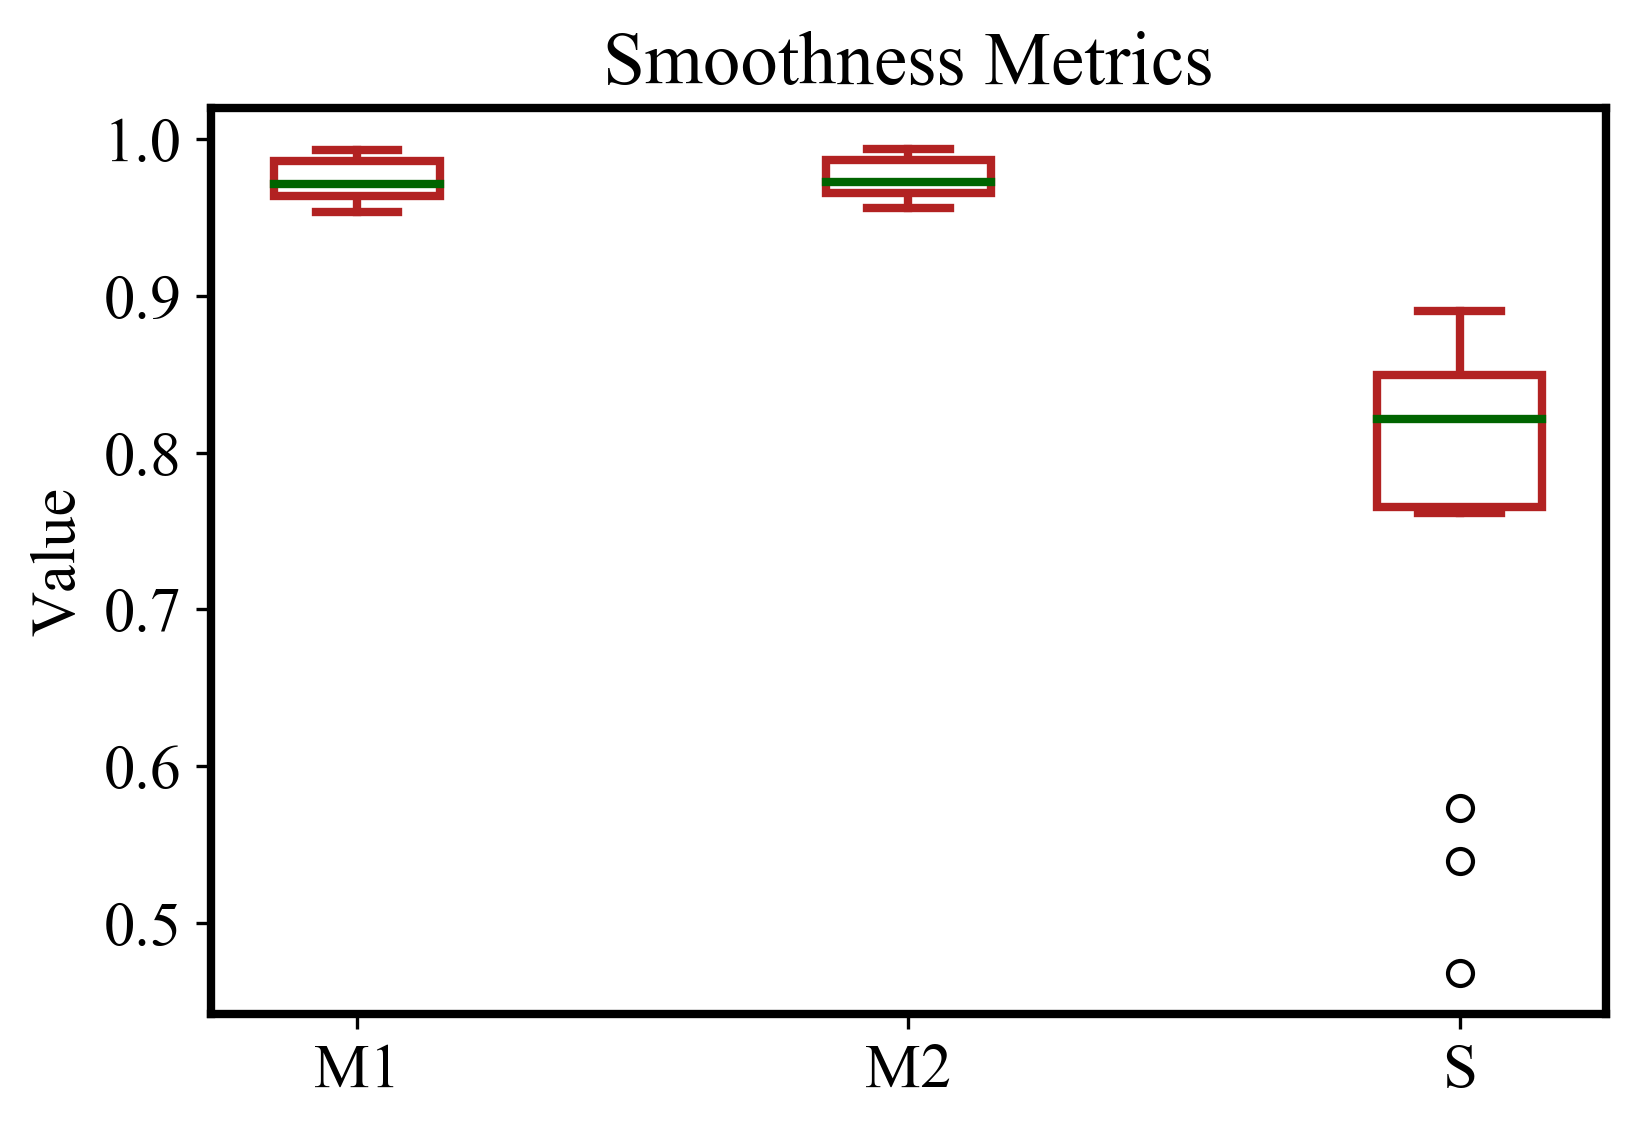
\includegraphics[width=0.7\textwidth]{crffigs/smooth.png}
    \caption{\label{fig:smooth} The three smoothness metrics $M1$, $M2$, $S$ evaluated on 15 validation predictions on PDNA-74 dataset. $S$ clearly behaves much nicer showing a large range of values compared to the rest.}
\end{figure}
Since, we want to implement it as a network layer, we define our terminology thus: Let, $B_i \in
\bR^d \;\forall i \in V$ be output of a neural network layer and is input the CCRF layer, $H_i \in
\bR^d \; \forall i \in V$ be output of the CCRF layer. In this scenario, we can think $B$ as analogous
to $x$ in eq. \ref{crf_general} and before any kind of optimization $H = H^0 = B$ is analogous to $y$ in
eq. \ref{crf_general}. $H$ then gets reassigned some final output value after the layer performs its
operation. Now, all variables are in continuous domain and the model looks as follows:
\begin{align*}
        P(H_i | B) &= 
        \frac{1}{Z(B)} exp [- (\psi_1(H_i,B_i) + \sum_{j \in
        \cN(i)}\psi_2(H_i,H_j,B_i,B_j)) ] \numberthis \label{ccrf}
\end{align*}
Now, it is time to design $\psi_1$ and $\psi_2$ which is straightforward in this case. We want
output $H_i$ to preserve its identity as much possible i.e. be as close to $B_i$ as possible, which
makes squared error w.r.t. a reasonable choice for $\psi_1$. However, we want $H_i$ to be not too
different from its neighbours also. We would like to different neighbours of $i$ differently
according to their initial similarity with vertex $i$. Finally, the two potential terms need to be
weighted by some optimizable constants determined by the network while training. This motivates the following choices of the functions:
\begin{align*}
        \psi_1(H_i, B_i) = \alpha ||H_i - B_i||_2^2 &\;\;\; \psi_2(H_i, H_j, B_i, B_j) = \beta
        g_{ij} ||H_i - H_j||_2^2 \;\; \alpha, \beta > 0 \\
        \text{A simple and effective choice: } & g_{ij} =
        exp\bigg{[}\frac{B_i^TB_j}{\sigma^2 ||B_i||_2||B_j||_2}\bigg{]} \;\; \numberthis 
\end{align*}
$\sigma$ in the above equation can be left to the network to optimize. There can be other choices of
$g_{ij}$ in the above equation too e.g. it can be parametrized as a separate neural network
itself.
This makes the final form of our CCRF model as follows:
\begin{align*}
        P(H_i | B) &= \frac{1}{Z(B)} exp [-(||H_i - B_i||_2^2 + \sum_{j \in
        \cN(i)} g_{ij} ||H_i - H_j||_2^2)] \numberthis \label{ccrf_final}
\end{align*}
Now, we need to optimize eq. \ref{ccrf_final} mathematically to get an update algorithm that the
network layer can execute to get the final result $\hat{H}$. For this, we turn to Bayesian Variational
Inference. In this framework, we propose to approximate the posterior distribution $P(H_i |
B)$ which may not have a tractable form, using a candidate distribution $Q(H)$ which has a suitable
form which we can work with. 
We can do this in this case, by adopting the standard mean field variational inference (VI) assumption
where we assume the full posterior distribution can be expressed as a product of independent
marginal distributions over the vertices. i.e. $Q(H) = \prod_{i \in V}Q_i(H_i)$. The we can minimize
the KL divergence between the candidate and target distribution is standard VI manner:
\begin{align*}
        Q^* = argmin_{Q \in \cQ} KL(Q(H) || P(H | B)) \numberthis \label{kl_div_min}
\end{align*}
Following mean field VI calculation presented in \cite{murphy2012machine}, we can now
calculate the posterior distribution of $H_i$:
\begin{align*}
Q^*_i(H_i) = \bE_{j\neq i}[ln P(H_i | B)] + const \numberthis \label{mean_field_VI_result}
\end{align*}
Now, the output of CCRF layer is simply the $\hat{H}_i$ that maximises $Q^*(H_i) \forall i \in V$.
Our detailed calculations for the same is presented in \hyperref[crf_detailed]{Appendices}. In essence, this constitutes a
system of equations over the vertices which can be solved by iteratively updating the vertices until
convergence is reached. For our purposes we stop the iterations at a set max iteration number T.
\hyperref[algo:CCRF_LAYER]{Algorithm 1} presents the final form of the CCRF layer as used in PNAbind.
The network optimizes the parameters $\alpha, \beta$ and $\sigma$. Intuitively, if the
input vertex information is already smooth and no update is necessary then $\beta$ goes towards 0 and 
otherwise, we have some non zero value of $\beta$ resulting in a balance between preserving the
vertex's own features and conforming to features of its neighbours. In the following section, we
show that using this layer as the second last of PNAbind significantly improves the smoothness of
predicted labels over protein meshes while improving upon or at least preserving desired 
metrics of classification results. Note: this is important, because a naive way to increase
smoothness of prediction is to predict the same class for all vertices, but, that would dramatically
decrease performance metrics of the prediction. \hyperref[fig:ccrf]{Fig. 1.3AB} schematically
describes the usage context and layer details of the CCRF layer as described in this section.
\begin{pmialgorithm}[0.9\textwidth]{h!}{CCRF Layer}\vskip-2ex
        \label{algo:CCRF_LAYER}
        \begin{algorithmic}[1]
                \REQUIRE  $B_i$  $\forall i$, $E$ (adjacency information)
                \STATE Initialize $H_i^0 = B_i$ $\forall i$\COMMENT{$H_i^0$ maximises $Q_i^0 = \frac{1}{Z_i^0}exp(-c||H_i^0 - B_i||^2)$}
                \FOR[$T$ signifies convergence]{$t=0,1,2,...,T-1$}
        \STATE compute $(\sum \limits_{j \in \mathcal{N}(i)} (g_{ij} H_j^t),\sum \limits_{j \in \mathcal{N}(i)} g_{ij})$ \COMMENT{message passing}
        \STATE $H_i^{t'} = \alpha B_{i} + \beta  \sum\limits_{j \in \mathcal{N}(i)} (g_{ij} H_j^t)$
        \STATE $H_i^{t+1} = H_i^{t'} / (\alpha +  \beta  \sum \limits_{j \in \mathcal{N}(i)} g_{ij} )$
                \ENDFOR
                \STATE $H_i^* = H_i^T$
                \RETURN $H_i^*$
        \end{algorithmic}
\end{pmialgorithm}
